\documentclass[border=4pt]{standalone}

\usepackage{amsmath}
\usepackage{tikz}
\usepackage{mathdots}
\usepackage{yhmath}
\usepackage{cancel}
\usepackage{color}
\usepackage{siunitx}
\usepackage{array}
\usepackage{multirow}
\usepackage{amssymb}
\usepackage{gensymb}
\usepackage{tabularx}
\usepackage{booktabs}
\usetikzlibrary{fadings}
\usetikzlibrary{patterns}
\usetikzlibrary{shadows.blur}
\usetikzlibrary{shapes}
 

\begin{document}


\tikzset{every picture/.style={line width=0.75pt}} %set default line width to 0.75pt        

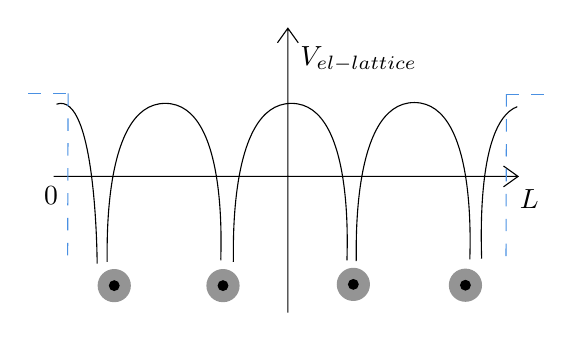
\begin{tikzpicture}[x=0.75pt,y=0.75pt,yscale=-1,xscale=1]
%uncomment if require: \path (0,300); %set diagram left start at 0, and has height of 300

%Shape: Circle [id:dp6663067094575839] 
\draw  [draw opacity=0][fill={rgb, 255:red, 0; green, 0; blue, 0 }  ,fill opacity=0.42 ] (116.44,183.01) .. controls (116.44,178.59) and (120.02,175.01) .. (124.44,175.01) .. controls (128.86,175.01) and (132.44,178.59) .. (132.44,183.01) .. controls (132.44,187.43) and (128.86,191.01) .. (124.44,191.01) .. controls (120.02,191.01) and (116.44,187.43) .. (116.44,183.01) -- cycle ;
%Shape: Circle [id:dp25474416249659915] 
\draw  [fill={rgb, 255:red, 0; green, 0; blue, 0 }  ,fill opacity=1 ] (122.1,183.01) .. controls (122.1,181.72) and (123.15,180.68) .. (124.44,180.68) .. controls (125.73,180.68) and (126.77,181.72) .. (126.77,183.01) .. controls (126.77,184.3) and (125.73,185.34) .. (124.44,185.34) .. controls (123.15,185.34) and (122.1,184.3) .. (122.1,183.01) -- cycle ;

%Shape: Axis 2D [id:dp09713278543252035] 
\draw  (42.8,130.4) -- (266.6,130.4)(155.69,59) -- (155.69,196) (259.6,125.4) -- (266.6,130.4) -- (259.6,135.4) (150.69,66) -- (155.69,59) -- (160.69,66)  ;
%Shape: Circle [id:dp9861405190620747] 
\draw  [draw opacity=0][fill={rgb, 255:red, 0; green, 0; blue, 0 }  ,fill opacity=0.42 ] (179.24,182.41) .. controls (179.24,177.99) and (182.82,174.41) .. (187.24,174.41) .. controls (191.66,174.41) and (195.24,177.99) .. (195.24,182.41) .. controls (195.24,186.83) and (191.66,190.41) .. (187.24,190.41) .. controls (182.82,190.41) and (179.24,186.83) .. (179.24,182.41) -- cycle ;
%Shape: Circle [id:dp9748843364258248] 
\draw  [fill={rgb, 255:red, 0; green, 0; blue, 0 }  ,fill opacity=1 ] (184.9,182.41) .. controls (184.9,181.12) and (185.95,180.08) .. (187.24,180.08) .. controls (188.53,180.08) and (189.57,181.12) .. (189.57,182.41) .. controls (189.57,183.7) and (188.53,184.74) .. (187.24,184.74) .. controls (185.95,184.74) and (184.9,183.7) .. (184.9,182.41) -- cycle ;

%Shape: Circle [id:dp7961136033324678] 
\draw  [draw opacity=0][fill={rgb, 255:red, 0; green, 0; blue, 0 }  ,fill opacity=0.42 ] (233.24,182.81) .. controls (233.24,178.39) and (236.82,174.81) .. (241.24,174.81) .. controls (245.66,174.81) and (249.24,178.39) .. (249.24,182.81) .. controls (249.24,187.23) and (245.66,190.81) .. (241.24,190.81) .. controls (236.82,190.81) and (233.24,187.23) .. (233.24,182.81) -- cycle ;
%Shape: Circle [id:dp5533581569571397] 
\draw  [fill={rgb, 255:red, 0; green, 0; blue, 0 }  ,fill opacity=1 ] (238.9,182.81) .. controls (238.9,181.52) and (239.95,180.48) .. (241.24,180.48) .. controls (242.53,180.48) and (243.57,181.52) .. (243.57,182.81) .. controls (243.57,184.1) and (242.53,185.14) .. (241.24,185.14) .. controls (239.95,185.14) and (238.9,184.1) .. (238.9,182.81) -- cycle ;

%Shape: Circle [id:dp8630120270700654] 
\draw  [draw opacity=0][fill={rgb, 255:red, 0; green, 0; blue, 0 }  ,fill opacity=0.42 ] (64.04,183.01) .. controls (64.04,178.59) and (67.62,175.01) .. (72.04,175.01) .. controls (76.46,175.01) and (80.04,178.59) .. (80.04,183.01) .. controls (80.04,187.43) and (76.46,191.01) .. (72.04,191.01) .. controls (67.62,191.01) and (64.04,187.43) .. (64.04,183.01) -- cycle ;
%Shape: Circle [id:dp4927013269724416] 
\draw  [fill={rgb, 255:red, 0; green, 0; blue, 0 }  ,fill opacity=1 ] (69.7,183.01) .. controls (69.7,181.72) and (70.75,180.68) .. (72.04,180.68) .. controls (73.33,180.68) and (74.37,181.72) .. (74.37,183.01) .. controls (74.37,184.3) and (73.33,185.34) .. (72.04,185.34) .. controls (70.75,185.34) and (69.7,184.3) .. (69.7,183.01) -- cycle ;

%Curve Lines [id:da2361557286551046] 
\draw    (68.6,171.6) .. controls (69,171.6) and (65,95.2) .. (96.6,95.2) .. controls (128.2,95.2) and (123,171.6) .. (123.4,170.8) ;
%Curve Lines [id:da6793229314687435] 
\draw    (129.4,171.6) .. controls (129.8,171.6) and (125.8,95.2) .. (157.4,95.2) .. controls (189,95.2) and (183.8,171.6) .. (184.2,170.8) ;
%Curve Lines [id:da19733766248470808] 
\draw    (188.6,171.2) .. controls (189,171.2) and (185,94.8) .. (216.6,94.8) .. controls (248.2,94.8) and (243,171.2) .. (243.4,170.4) ;
%Curve Lines [id:da255362719510541] 
\draw    (249,170) .. controls (249.4,170.8) and (245,104.8) .. (266.2,96.8) ;
%Curve Lines [id:da5345088985354827] 
\draw    (44.2,95.6) .. controls (63.4,88.8) and (63.8,171.2) .. (63.8,172.4) ;
%Straight Lines [id:da5838524100568929] 
\draw [color={rgb, 255:red, 74; green, 144; blue, 226 }  ,draw opacity=1 ] [dash pattern={on 4.5pt off 4.5pt}]  (261,90.8) -- (260.8,170.2) ;
%Straight Lines [id:da5155413480528697] 
\draw [color={rgb, 255:red, 74; green, 144; blue, 226 }  ,draw opacity=1 ] [dash pattern={on 4.5pt off 4.5pt}]  (49.8,90.4) -- (49.6,169.8) ;
%Straight Lines [id:da5252520282026882] 
\draw [color={rgb, 255:red, 74; green, 144; blue, 226 }  ,draw opacity=1 ] [dash pattern={on 4.5pt off 4.5pt}]  (261,90.8) -- (280.2,90.8) ;
%Straight Lines [id:da23005361103874167] 
\draw [color={rgb, 255:red, 74; green, 144; blue, 226 }  ,draw opacity=1 ] [dash pattern={on 4.5pt off 4.5pt}]  (30.6,90.4) -- (49.8,90.4) ;

% Text Node
\draw (272,141.4) node    {$L$};
% Text Node
\draw (41.6,139.6) node    {$0$};
% Text Node
\draw (192,74) node    {$V_{el-lattice} \ $};


\end{tikzpicture}


\end{document}
